% !TeX encoding = UTF-8
% !TeX spellcheck = en_US
\documentclass[twocolumn]{article}
\usepackage[cm]{fullpage}
\usepackage{moodlev5}
\usepackage{tikz}
\usepackage{varwidth}
\usepackage{multirow,hyperref}
\usepackage{colortbl,threeparttable}

\def\myequation{y=a\sqrt{x}+b}

\tikzstyle{pict} = [minimum height=1em,inner sep=0pt,execute at begin 
node={\begin{varwidth}{\linewidth}},
execute at end node={\end{varwidth}}]

\newcommand\pictembedding[1]{\begin{tikzpicture}\node[pict]{#1};\end{tikzpicture}}

\htmlregister{\myequation}
\htmlregister{\pictembedding}

\begin{document}

\section*{Introduction}

This document presents examples of questions that one can make with the 
\texttt{moodle} \LaTeX{} package as of version \texttt{0.5}, currently 
available on \href{https://ctan.org/pkg/moodle}{CTAN}.

\begin{table*}[tbp]
\centering
\begin{threeparttable}[b]
\caption{Question types and content enrichment capabilities after XML import in 
moodle \texttt{v3.1}.}
\label{tab:2}
\begin{tabular}{rl|ccc|ccc}
\multicolumn{2}{c|}{}& \multicolumn{3}{c|}{\LaTeX{} rendering} & 
\multicolumn{3}{c}{Picture embedding}\\
\multicolumn{2}{c|}{Question type}& Question & Answer & Feedback & Question & 
Answer & Feedback\\\hline\hline

&\href{https://docs.moodle.org/31/en/Multiple_Choice_question_type}{Multichoice}\tnote{1}
 & \cellcolor{green}  & \cellcolor{green} & \cellcolor{red}no \LaTeX\tnote{2}
 & \cellcolor{green} & \cellcolor{green} & \cellcolor{red}no 
 \LaTeX\tnote{2}\\\hline

& \href{https://docs.moodle.org/31/en/Numerical_question_type}{Numerical} & 
\cellcolor{green} & \cellcolor{black!25}Text only\tnote{5} & \cellcolor{red}no 
\LaTeX\tnote{2} & \cellcolor{green} & \cellcolor{black!25}Text only\tnote{5} & 
\cellcolor{red}no \LaTeX\tnote{2}\\\hline

& \href{https://docs.moodle.org/31/en/Short-Answer_question_type}{Short Answer} 
& \cellcolor{green} & \cellcolor{black!25}Text only\tnote{5} & 
\cellcolor{red}no \LaTeX\tnote{2} & \cellcolor{green} & 
\cellcolor{black!25}Text only\tnote{5} & \cellcolor{red}no 
\LaTeX\tnote{2}\\\hline

&Matching 
(\href{https://docs.moodle.org/31/en/Matching_question_type}{standard}) & 
\cellcolor{green} & \cellcolor{black!25}Text only\tnote{3} & 
\cellcolor{black!25}Irrelevant\tnote{4} & \cellcolor{green} & 
\cellcolor{black!25}Text only\tnote{3} & 
\cellcolor{black!25}Irrelevant\tnote{4} \\\hline

&Matching 
(\href{https://docs.moodle.org/31/en/Drag_and_drop_matching_question_type}{drag-and-drop})
 & \cellcolor{green} & \cellcolor{green} &\cellcolor{black!25} 
 Irrelevant\tnote{4} & \cellcolor{green} & \cellcolor{green} &  
 \cellcolor{black!25} Irrelevant\tnote{4} \\\hline

&\href{https://docs.moodle.org/31/en/Essay_question_type}{Essay}\tnote{8} & 
\cellcolor{green} & \cellcolor{orange}note\tnote{6}, bug\tnote{9} & 
\cellcolor{black!25}Irrelevant\tnote{7} & \cellcolor{green} & 
\cellcolor{orange}note\tnote{6}, bug\tnote{9} & 
\cellcolor{black!25}Irrelevant\tnote{7}\\\hline

\multirow{5}{*}{\href{https://docs.moodle.org/31/en/Embedded_Answers_(Cloze)_question_type}{Cloze}}
 &Numerical&\checkmark & \cellcolor{black!25}Text only\tnote{5} & No & 
 \checkmark & 
\cellcolor{black!25}Text only\tnote{5} & 
\checkmark\\\cline{2-8}
&Short Answer&\checkmark & \cellcolor{black!25}Text only\tnote{5} & No & 
\checkmark & \cellcolor{black!25}Text only\tnote{5} & 
\checkmark\\\cline{2-8}
&Multi (dropdown) &\checkmark & \cellcolor{black!25}Text only\tnote{3} & No & 
\checkmark & \cellcolor{black!25}Text only\tnote{3} & \checkmark\\\cline{2-8}
&Multi (horizontal)& \checkmark & \checkmark & No & \checkmark & \checkmark & 
\checkmark\\\cline{2-8}
&Multi (vertical)& \checkmark & \checkmark & No & \checkmark & \checkmark & 
\checkmark\\\hline
\end{tabular}
\begin{tablenotes}
\item[1] Numbering with option ``ABC" is not recognized by moodle after XML 
import.
\item[2] \LaTeX{} code here tends to break the compilation of the document. 
Probably because of the symbol $\backslash$ or $\{$.
\item[3] Moodle uses a dropdown list to let the user choose among the 
possible answers. This forbids either pictures and \LaTeX{} rendering.
\item[4] Not supported by moodle (in this context, answer-specific feedback 
represents lots of possible combinations).
\item[5] Moodle uses a HMTL input tag to let the user enter his answer. This 
forbids pictures and \LaTeX{} rendering.
\item[6] In the context of this package, answers represent ``notes for the 
grader" while ``template" represents suggested contents as a starting point.
\item[7] For obvious reasons, essays cannot be graded automatically.
\item[8] The keyval ``response template", as documented, is broken. Works if 
replaced with ``template".
\item[9] Picture and LaTeX rendering could be done, but only after submission 
and only if the keyval "response format" was set to ``html". Unfortunately, the 
\texttt{<p>...</p>} tags introduced, whatever the response format is, prevent 
rendering.
\end{tablenotes}
\end{threeparttable}
\end{table*}

\begin{quiz}[ % options that apply to all questions
%	points=1, % default 1
%	penalty=0, % penalty in case of wrong attempt (between 0 and 1). Default 0.1
%	fraction=0, % fraction of points for wrong or partially true answers
	%feedback={coucou}
	] {Example Quiz}

\begin{multi}[points=3,numbering=Alph]{Multiple Choice (single correct answer)}
% Numbering possibilities:
% - numbering=alph, alpha, or abc,
% - numbering=Alph, Alpha, or ABC, (broken at XML import)
% - numbering=arabic or 123,
% - numbering=roman or iii,
% - numbering=Roman or IIII,
% - numbering=none.
	What is the first derivative of $x^3$ w.r.t. $x$?
	\item[feedback={this is a very long feedback; it may even be displayed in 
		several lines. Here is a new sentence! Does that work? Yes.}] 
		$\frac{1}{4} x^4+C$
	\item[]* $3x^2$ % the star stands for fraction=1
	\item[feedback={text}] $51$
\end{multi}

\begin{multi}[multiple,numbering=roman]{Multiple Choice (several correct 
		answers)} % 
	Select the following numbers that are prime.
	\item[feedback={it is only divided by 1 and itself!}]* 5
	\item[feedback={divided by 2 and 3!}] 6
	\item[]* 7 %feedback={it is only divided by 1 and itself!}
	\item[feedback={divided by 2 and 4! Normally this feedback would be short 	
		but I want to make it longer for testing purposes.}] 8
\end{multi}

\begin{numerical}[ % options that apply to all answers
%	points=1, % default 1
%	penalty=0, % penalty in case of wrong attempt (between 0 and 1). Default 0.1
%%	fraction=0, % fraction of points for wrong or partially true answers
%	feedback={coucou} % feedback is given regardless of the answer
	] {Numerical}
What is $8+3$?
\item[fraction=100,feedback={this is a very long feedback; it may even be 
displayed in several lines. Here is a new sentence! Does that work? Yes.}] $11$
\item[fraction=0] 12
\item[fraction=0,feedback={Pfff}] 5
\end{numerical}

\begin{shortanswer}[case sensitive=true]{Short Answer (case sensitive)}
What was Newton's first name?
\item[feedback={this is a very long feedback; it may even be displayed in 
several lines. Here is a new sentence! Does that work? Yes.}] Isaac
\item[fraction=50,feedback={forgot how to capitalize properly?}] isaac
\item[fraction=0] Fig Fag Fog
\item[fraction=0,feedback={how noble!}] Sir
\end{shortanswer}

\begin{shortanswer}{Short Answer (case insensitive)}
Newton's rival was Gottfried Wilhelm \blank.
\item[feedback={Correct! But why the hell did you put a dot?}] Leibniz.
\item Leibniz
\item[fraction=0,feedback={write it backwards!}] Zinbiel
\end{shortanswer}

\begin{matching}{Matching (standard)}
Answer-specific feedback is too complicated for matching questions (lots of 
possible combinations). Moodle does not support that\dots

In moodle, the matching is made by selecting answers in a dropdown list. The 
latter only allows text: pictures cannot be placed and neither HTML nor LaTeX 
are rendered. 
	\item[feedback={this feedback is garbage: it is placed in the XML but won't 
	make it through the moodle import}] Orange \answer Orange
	\item[feedback={Actually, moodle's matching question type does not seem to 
	support feedback}] $Lemon\quad\myequation$ \answer Yellow
	\item[feedback={sadly...}] Banana \answer Yellow
% "Yellow" is repeated twice but will appear only once in the offered answers
	\item[] Strawberry \answer Red
	\item[]  \answer Black
\end{matching}

\begin{matching}[dd]{Matching (drag and drop)}
This question type comes with a specific moodle plugin. In the offered answers, 
it allows to place pictures and get HTML or LaTeX 
rendered.\pictembedding{$\myequation$}
	\item[feedback={this feedback is garbage: it is placed in the XML but won't 
	make it through the moodle import}] 
	Orange \answer $Orange$
	\item[feedback={Actually, moodle's matching question type does not seem to 
	support feedback}] $Lemon\quad\myequation$ \answer Yellow
	\item[feedback={sadly...}] Banana \answer Yellow
% "Yellow" is repeated twice but will appear only once in the offered answers
	\item[] Strawberry \answer Red
	\item[]  \answer Black $\myequation$
\end{matching}

\begin{essay}[response required,response 
format=text,template={test $\myequation$}]{Essay}
Is learning worth it?
\item if the answer is "yes" $\rightarrow$ full grade
\item if the answer is silly  $\rightarrow$ minimum grade
\end{essay}

\begin{cloze}{Cloze}
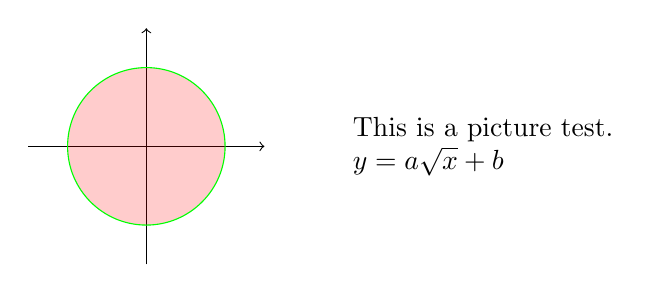
\begin{tikzpicture}
\draw[->] (-1.5,0)--(1.5,0);
\draw[->] (0,-1.5)--(0,1.5);
\draw[fill=red,fill opacity=.2,draw=green] (0,0)circle[radius=1];
\node[text width=3.5cm,anchor=west] at (2.5,0) {This is a picture test. 
$\myequation$};
\end{tikzpicture}
Within the cloze environment, when using multichoice, moodle allows to make 
only one choice. Therefore, multiple choice questions shall be made such that 
all points can be acquired with a single good answer only. A limitation of 
moodle's parser, discussed 
\href{https://moodle.org/mod/forum/discuss.php?d=275299}{here}, has to be 
overcome for math display in answers or feedbacks that contain closing curly 
braces ($\}$). It should be escaped with a $\backslash$.

\begin{multi}
First, an inline dropdown list. It is very compact on moodle. The drawback is 
that there is no LaTeX or HTML rendering in answers. The feedback renders HMTL 
and LaTeX. It is a bit hidden as it pops up only when hovering the 
checkmark or X mark with the mouse.
\item[feedback={yes}]* chip
\item[fraction=10] chop
\item[feedback={this is a quite long feedback.}] chap
\end{multi}

\begin{multi}[horizontal]
Second, an horizontal multichoice. May be quite compact as well but inadequate 
when possible answers are lengthy or numerous. Both answers and feedback can 
be rendered using LaTeX and HTML.
\item[feedback={text}]* True
\item[] False
\item[feedback={silly!}] $Dunno$
\end{multi}

\begin{multi}[vertical]
Last, a vertical multichoice. Behaves like the standard single multichoice.
\item[feedback={yes!}]* yop
\item[fraction=20] yap
\item[feedback={no!}] yip
\item[feedback={nope...}] $yup$
\end{multi}
\end{cloze}

\end{quiz}

%\begin{quiz}{Second Quiz}	
%\begin{numerical}{Numerical}
%What is $1+1$?
%\item 2
%\end{numerical}	
%\end{quiz}

\end{document}